\documentclass[12pt]{article}

\usepackage[english, italian]{babel}
\usepackage[letterpaper,top=2.5cm,bottom=2.5cm,left=2.5cm,right=2cm,marginparwidth=1.75cm]{geometry}
\usepackage{amsmath}
\usepackage{graphicx}
\usepackage{csquotes}
\usepackage{multirow}
\usepackage[colorlinks=true, allcolors=blue]{hyperref}
\usepackage[backend=biber, style=ieee]{biblatex}
\usepackage[ruled, vlined]{algorithm2e}
\usepackage{url} %citazioni di wikipedia più belle
\usepackage[bottom]{footmisc} %footnote in fondo alla pagina
\usepackage{placeins} %FloatBarrier

\usepackage{listings}

%%Macro personali
\newcommand{\quotes}[1]{``\textit{#1}''}
\newcommand{\virg}[1]{``#1''}

\graphicspath{{./immagini/}}

\author{
  Stefano Travasci\\
  Mat. 133014\\
  \texttt{travasci.stefano@spes.uniud.it} \and
  Riccardo Zamolo\\
  Mat. 135047 \\
  \texttt{zamolo.riccardo@spes.uniud.it}
}
\date{}

\addbibresource{bibliography.bib}

\title{
    Università degli Studi di Udine \\
    Dipartimento di Scienze Matematiche, Informatiche e Fisiche \\
    \vspace{50pt}
    Relazione progetto per il corso di Architetture parallele \\
    A.A. 2022/2023
    \vspace{50pt}
    \begin{center}
        
\includegraphics[scale=0.1]{uniud.png}
    \end{center}
    \vspace{50pt}
    \textbf{Individuazione di tutti i matching per il problema dei matrimoni stabili}
    \vspace{50pt}
}


\begin{document}

\begin{titlepage}
\maketitle
\thispagestyle{empty}
\end{titlepage}

\tableofcontents
\listoffigures

\pagebreak

\section{Introduzione}
    La presente relazione ha come obiettivo quello di presentare una soluzione algoritmica seriale e una parallela (sfruttando l'estensione CUDA del linguaggio di programmazione C) per una estensione del problema dei matrimoni stabili. In particolare, si richiede di trovare tutti i possibili matching stabili e non soltanto uno solo, come invece previsto dalla forma classica del problema.
    
    \subsection{Il problema dei matrimoni stabili}
        Il problema dei matrimoni stabili\cite{StableMarriageProblem} consiste nel trovare un \textbf{matching stabile} tra due insiemi aventi la stessa cardinalità, basandosi sulle preferenze espresse da ciascun elemento dei due insiemi. Un \textbf{matching}, nel contesto del problema in esame, consiste nella creazione di una serie di accoppiamenti tra insiemi del primo e del secondo insieme. Il numero di coppie presenti nel matching sarà uguale alla cardinalità degli insiemi. Un matching è \textbf{stabile} se non esiste alcuna coppia $(A,B)$ tale che $A$ preferisce $B$ al suo attuale partner e viceversa. Se invece esiste almeno una tale coppia, allora il matching si dice instabile.
        
        Per facilitare la comprensione del problema, si può sfruttare la metafora dei matrimoni: dati $n$ uomini e $n$ donne, si richiede di creare $n$ coppie uomo-donna (matrimoni), tali per cui non esistono coppie uomo-donna che si preferiscono a vicenda rispetto ai loro attuali partner.

    \subsection{Estensioni del problema}
        Esistono svariati problemi simili a quello dei matrimoni stabili, come per esempio lo \textit{stable roommates problem}\cite{StableRoommatesProblem}, in cui l'unica differenza è che gli elementi non vengono suddivisi in due insiemi, ma appartengono tutti allo stesso pool iniziale. Generalizzazioni di questo problema permettono di imporre delle condizioni ai matching, ad esempio coppie che devono necessariamente essere incluse o escluse oppure membri di un gruppo che devono essere accoppiati allo stesso elemento. Altro tipo di generalizzazione è quello che estende la cardinalità del problema da \textit{one-to-one} (un uomo per ogni donna, e viceversa) a cardinalità di tipo \textit{one-to-many} o \textit{many-to-many}. Ad esempio nel \textit{rural hospitals theorem}\cite{RuralHospitals} dei dottori devono essere assegnati a degli ospedali: ogni ospedale ha più di un posto disponibile e solitamente il numero di posti disponibili è superiore a quello dei dottori; inoltre alcuni partecipanti potrebbero essere disposti ad essere assegnati solo ad un sottoinsieme dei membri dell'altro lato del matching. Si hanno ulteriori variazioni del problema a seconda che l'ordinamento delle preferenze sia stretto, per cui non è possibile che il membro di un gruppo valuti due alternative come equivalenti, oppure non stretto, quando in una lista di preferenze alcune alternative possono essere valutate come qualitativamente equivalenti; nel secondo caso si parla di \textit{stable marriage with indifference}.\cite{StableMarriageIndifference} Nel presente testo vogliamo calcolare tutti i matching stabili relativi a un'istanza del problema classico, in cui ogni elemento fa parte di una e una sola coppia (\textit{one-to-one}) e le preferenze sono ordinate in modo stretto.

    \subsection{Trovare tutte le soluzioni} \label{TrovareTutteLeSoluzioni}
    In questo lavoro affrontiamo il problema di trovare tutte le possibili soluzioni ad una particolare istanza del problema dei matrimoni stabili, con le preferenze espresse con un ordine stretto.
    
    Sappiamo da \cite{irving1986complexity} che l'enumerazione di tutti i matching stabili è un problema \#P-completo.\footnote{Da \cite{irving1986complexity}: \quotes{The concept of \#P-completeness was introduced by Valiant [...] in order to describe those enumeration problems that are \virg{at least as hard} as NP-complete problems.}} Essendo il conteggio dei matching stabili \#P-completo, lo deve essere anche elencarli. Scendendo più in dettaglio per quanto riguarda il numero di soluzioni, \cite{9719708} trova un upper bound di $O(3,55^n)$ e \cite{THURBER2002195} trova dei lower bound comunque esponenziali. Ne segue che un qualsiasi algoritmo che trovi tutte le soluzioni debba impiegare un tempo almeno esponenziale.
    
    Fra i lavori precedenti che hanno trattato il nostro stesso problema, menzioniamo \cite{McVitie1971}, \cite{ThreeProcedures1971} e \cite{Gusfield3FastAlg}. \cite{DIAS2003391}, \cite{EirinakisEtAl2012} e \cite{gutin2023finding} si occupano invece di trovare tutte le soluzioni in variazioni del problema originale.

    Si noti che alcuni lavori, come \cite{cai2019representing}, si occupano di trovare una rappresentazione implicita dei risultati attraverso il grafo delle rotazioni. In questo lavoro faremo anche il passo successivo, ricavando l'elenco esplicito di tutti i matching stabili.
        
\pagebreak

\section{Soluzione seriale}

    Nella sezione corrente si presentano prima le nozioni teoriche e la soluzione algoritmica seriale ad alto livello. Quindi sono introdotte le strutture dati utilizzate e, infine, lo pseudocodice della soluzione.
    
    \subsection{Le basi teoriche}
    L'insieme delle soluzioni al problema dei matrimoni stabili può essere articolato in un reticolo (\textit{lattice of stable matchings}) i cui elementi sono le singole soluzioni.\cite{LatticeOfStableMatchings} Una rotazione è l'insieme dei cambiamenti necessari per trasformare un matching in un altro matching ad esso adiacente nel reticolo. Inoltre, dato un matching, una rotazione si dice \textit{esposta} qualora sia possibile applicarla al matching. In ogni matching stabile, una rotazione può essere esposta o meno. Si considerino ad esempio i seguenti matching stabili $M_i$ e $M_{i+1}$

    \begin{center}
        $M_i = \bigg\{ (1, 2), (2, 3), (3, 1), (4, 4) \bigg\}$
        \hspace{10pt}
        \begin{center}
        $M_{i+1} = \bigg\{ (1, 3), (2, 2), (3, 1), (4, 4) \bigg\}$
        \end{center}    
    \end{center}

    I cambiamenti necessari per passare da $M_i$ a $M_{i+1}$ costituiscono una rotazione $\rho$, così definita  
    
    \begin{center}
        $\rho = (1, 2), (2, 3)$    
    \end{center}

    I matching in cima e in fondo al reticolo dei matching stabili sono, rispettivamente, la soluzione ottimale per gli uomini (e peggiore per le donne) e quella ottimale per le donne (e peggiore per gli uomini). Entrambe possono essere calcolate in tempo $O(n^2)$ usando l'algoritmo di Gale–Shapley.\cite{GaleShapley} Per calcolare il matching in fondo è sufficiente invertire il ruolo degli uomini e delle donne nell'algoritmo di Gale–Shapley. Si noti che, a causa dell'inversione dell'ordine dei parametri, se il matching è rappresentato come un vettore, il significato di indici e valori sarà invertito; è possibile facilmente invertire nuovamente indici e valori in tempo $O(n)$.

    \subsection{Descrizione generale}
    \label{DescrizioneGeneraleSeriale}
    L'idea alla base del nostro algoritmo è partire dal matching migliore per gli uomini ed esplorare il reticolo delle soluzioni dall'alto verso il basso attraverso una depth-first search, spostandoci ogni volta di una singola rotazione.
    
    Per fare ciò in modo efficiente, troviamo tutte le rotazioni e successivamente, costruiamo un grafo che codifica le dipendenze fra le rotazioni. Per compiere entrambi gli step, seguiamo gli algoritmi proposti in \cite{Gusfield3FastAlg} e \cite{GusfieldBook}. In particolare, per trovare le rotazioni è stato implementato l'algoritmo descritto ad alto livello nel terzo paragrafo di \cite{Gusfield3FastAlg}. Per costruire il grafo delle rotazioni ci si è basati sull'algoritmo descritto a pagina 112 di \cite{GusfieldBook}\footnote{Lo stesso algoritmo è descritto anche in \cite{Gusfield3FastAlg}, ma la spiegazione è molto più comprensibile nel libro.}, applicando una correzione. Come spiegato in \cite{cai2019representing}, infatti, l'algoritmo lì proposto contiene un errore. \cite{cai2019representing} propone un algoritmo alternativo, ma nell'appendice B identifica e propone una soluzione per l'algoritmo originale; pur trovando correttamente il punto in cui l'algoritmo di \cite{GusfieldBook} fallisce, la natura esatta dell'errore non è compresa correttamente, e dunque la soluzione proposta non è adeguata.

    Per risolvere questo errore, ci siamo basati sulla definizione di predecessori data in \cite{cai2019representing} (\textit{Definition 4.4})\footnote{Una definizione equivalente è data in \cite{GusfieldBook}, ma con una formulazione di difficile comprensione. È plausibile che proprio la formulazione poco chiara di questa definizione sia stata l'origine dell'errore nell'algoritmo.}. Studiando più accuratamente questa definizione, risulta evidente che l'algoritmo di \cite{GusfieldBook} verifica solo la prime delle due condizioni necessarie per identificare i predecessori di tipo 2. Dunque, per correggere l'algoritmo, abbiamo aggiunto, nella fase iniziale di etichettatura, una nuova sequenza di etichettature: così come nell'algoritmo originale scansioniamo la lista delle preferenze delle donne per aggiungere le etichette di tipo due, facciamo lo stesso per la lista di preferenze degli uomini. Nel passo successivo, verranno aggiunti solo gli archi di tipo due che sono stati etichettati due volte, ovvero sia scandendo la lista delle preferenze delle donne che quella degli uomini. Si noti che ogni coppia non stabile può essere etichettata al più due volte, una per ogni lista. Questa piccola modifica permette di aggiungere gli archi di tipo 2 che effettivamente rispettano entrambi i requisiti.
    
    Il grafo che costruiamo è simile a quello descritto nel terzo paragrafo di \cite{Irving1987AnEA}, con una piccola differenza: mentre quel grafo rappresenta la relazione di \textit{predecessore immediato} (\textit{immediate predecessor}) tra le rotazioni, nel nostro grafo alcuni archi sono ripetuti più volte. Questi archi possono essere facilmente rimossi, con una piccola modifica alla nostra soluzione. Si può facilmente notare che il grafo dei \textit{predecessori immediati} in \cite{Irving1987AnEA} è un sottografo di quello creato qui (in particolare, ha gli stessi nodi e un sottoinsieme degli archi). Entrambi i grafi sono funzionali per gli scopi di questo lavoro; mentre quello più piccolo permetterebbe successivamente di eseguire meno operazioni, quello più grande è più facile da calcolare e il numero maggiore di archi non aumenta la complessità asintotica dell'algoritmo.
    
    La ricerca effettiva di tutte le soluzioni è diversa da quella in \cite{Gusfield3FastAlg}, pur ispirandosi al concetto di ordinamento delle rotazioni lì presentato. Nonostante le differenze, i due approcci sono tuttavia alquanto simili e fondamentalmente equivalenti.

    Ogni chiamata di \texttt{RECURSIVE\_SEARCH} riceve come input un matching e una lista di rotazioni esposte rispetto a quel matching. Per ogni rotazione $\rho$ nella lista di rotazioni, essa viene applicata singolarmente al matching di input, ottenendo così un nuovo matching. Quindi viene effettuata una chiamata ricorsiva sul nuovo matching e sulla parte della lista di rotazioni successiva a $\rho$, a cui vengono aggiunte eventuali rotazioni rese esposte dall'applicazione di $\rho$; il significato di questo passo è il seguente: dopo aver trovato un nuovo matching applicando una rotazione $\rho$, si trovano tutti i matching ottenibili applicando le rotazioni che seguono $\rho$ nella lista delle rotazioni originale e le rotazioni che sono diventate esposte dopo l'applicazione di $\rho$. Si noti che non solo in questo modo vengono trovate tutti i possibili matching, ma che vengono inoltre trovati tutti una sola volta, rendendo superfluo controllare se il nuovo matching era stato già trovato in precedenza. Infatti, essendo escluse dalla chiamata ricorsiva le eventuali rotazioni che precedono la rotazione applicata nella lista, i successori non ancora esposti posso essere resi tali solo applicando i suoi predecessori nello stesso ordine in cui appaiono nella lista delle rotazioni. In altre parole, perché siano applicati tutti i predecessori, allora essi devono essere applicati nell'ordine definito dalla lista: ad esempio se applicassimo il secondo predecessore senza aver applicato il primo, nelle chiamate ricorsive successive il primo predecessore non sarà mai nella lista, dunque non sarà mai applicato e il successore non diventerà mai esposto. Partendo dal matching migliore per gli uomini e dalla lista delle rotazioni nel grafo che non hanno predecessori, viene così effettuata una visita DFS che definisce implicitamente un albero di copertura del reticolo dei matrimoni stabili.

    Si noti infine il gran numero di parametri delle funzioni: molti di essi non forniscono dati alle funzioni, ma passano delle strutture dati create in precedenza, permettendo di diminuire il consumo di memoria e soprattutto il numero di operazioni sulla memoria.

    \subsection{Le strutture dati}
    In questo paragrafo presentiamo le strutture dati principali usate nello pseudocodice. In particolare, per quanto riguarda le liste, le distinguiamo in due categorie: le liste \virg{semplici} e le liste \virg{complesse}. Le liste \virg{semplici} sono composte esclusivamente dagli elementi della lista, che contengono solo il proprio valore e un puntatore al prossimo elemento della lista (o in caso a \texttt{NULL}). Le liste \virg{complesse} invece permettono di accedere in tempo costante sia al primo che all'ultimo elemento della lista, in modo da rendere costante l'operazione di \texttt{append}; dal punto di vista realizzativo, una implementazione plausibile prevede l'utilizzo di liste \virg{semplici} per costruire le liste \virg{complesse}, che possono contenere semplicemente un puntatore al primo e all'ultimo elemento della lista. L'utilizzo di questi due tipi di liste permette di migliorare l'efficienza di alcune operazioni senza complicare eccessivamente il resto del codice.
    
    Di seguito si presenta un elenco più dettagliato di tutte le principali strutture dati utilizzate nello pseudocodice:

    \begin{itemize}
        \item \textbf{results\_list} è la struttura dati che contiene tutte le soluzioni del problema, ovvero tutti i matching stabili. Si tratta di una lista \virg{complessa} di puntatori ad array di interi, dove ogni array rappresenta un matching stabile (indici = uomini, valori = donne).
        \item \textbf{list\_el}: è una lista \virg{semplice} contente una rotazione, ogni elemento della lista (rotazione) è una coppia di interi uomo-donna.
        \item \textbf{rotation\_node}: è il nodo del grafo che rappresenta una rotazione. Ogni nodo è costituito dai campi: \texttt{rotation} - un puntatore alla lista della rotazione, \texttt{index} - l'indice intero univoco della rotazione, utilizzato per ridurre, con opportuni controlli, il numero di archi nel grafo delle rotazioni, \texttt{missing\_predecessors} - intero che tiene traccia dei predecessori mancanti, \texttt{successors} - la lista (\virg{semplice}) dei successori di questa rotazione.
        \item \textbf{free\_rotations\_list}: è la lista di rotazioni esposte rispetto a un particolare matching, ovvero la lista di nodi del grafo che non hanno predecessori. In termini implementativi, è una lista di puntatori a nodi del grafo. A seconda della funzione in cui appare, può essere usata come lista \virg{complessa} o come lista \virg{semplice}, utilizzando direttamente gli elementi della lista.
        
    \end{itemize}
        
    \subsection{L'algoritmo seriale}
    Di seguito si presenta lo pseudocodice seriale per l'enumerazione di tutti i matching stabili. Si noti che nello pseudocodice non vengono riportate le righe inerenti alla liberazione della memoria allocata delle strutture dati.

    
    \begin{algorithm}[H]
        \scriptsize
        \DontPrintSemicolon
        \caption{ALL\_STABLE\_MATCHINGS}\label{alg:AllStableMatchings}
        \KwData{n, men\_preferences, women\_preferences}
        \KwResult{results\_list}
        \;
        results\_list = NEW\_LIST\_EL()\;
        top\_matching = GALE\_SHAPLEY(n, men\_preferences, women\_preferences)\;
        inverted\_bottom\_matching = GALE\_SHAPLEY(n, women\_preferences, men\_preferences)\;
        bottom\_matching = int[n]\;
        \For{i = 0; i $<$ n} {
            bottom\_matching[inverted\_bottom\_matching[i]] = i\;
        }
        \;
        \texttt{//termina subito se non ci sono rotazioni}\;
        only\_one\_matching = true\;
        \For {i = 0; i $<$ n} {
            \If {top\_matching[i] $\ne$ bottom\_matching[i]} {
			only\_one\_matching = 0\;
			break\;
		}
        }
        \If{only\_one\_matching} {
            results\_list.first = NEW\_LIST\_EL()\;
		results\_list.first.value = top\_matching\;
		results\_list.first.next = NULL\;
		results\_list.last = results\_list.first\;
		\Return results\_list\;
        }
        \;
        \texttt{//copia top matching}\;
        top\_matching\_copy = int[n]\;
        \For{i = 0; i $<$ n}{
            top\_matching\_copy[i] = top\_matching[i]
        }
        \;
        \texttt{//crea la lista di rotazioni}\;
        rotations\_list = FIND\_ALL\_ROTATIONS(men\_preferences, women\_preferences, n, top\_matching\_copy, bottom\_matching)\;
        \;
        \texttt{//crea il grafo delle rotazioni}\;
        BUILD\_GRAPH(n, rotations\_list, top\_matching, men\_preferences, women\_preferences)\;
        \;
        \texttt{//calcolo la lista delle rotazioni libere}\;
        free\_rotations\_list = NEW\_EMPTY\_LIST()\;
        free\_rotations\_list.first = NULL\;
        free\_rotations\_list.last = NULL\;
        list\_el = rotations\_list.first\;
        \While{list\_el $\ne$ NULL}{
            \If{list\_el.value.missing\_predecessors == 0}{
                free\_rotations\_list.append(list\_el.value)\;
            }
            list\_el = list.el.next\;
        }
        \;
        \texttt{//aggiungo top matching ai risultati}\;
        results\_list.first = NEW\_LIST\_EL()\;
        \For (\tcp*[h]{per non lavorare sul matching salvato tra i risultati}){i = 0; i $<$ n}{
            top\_matching\_copy[i] = top\_matching[i]\;
        }
        results\_list.first.value = top\_matching\_copy\;
        results\_list.first.next = NULL\;
        results\_list.last = results\_list.first\;
        \;
        \If{rotations\_list.first $\ne$ NULL}{
            RECURSIVE\_SEARCH(top\_matching, n, free\_rotations\_list.first, results\_list)\;
        }
        \;
        \Return results\_list\;
    \end{algorithm}

    \begin{algorithm}[H]
        \scriptsize
        \DontPrintSemicolon
        \caption{GALE-SHAPLEY}\label{alg:GaleShapley}
        \KwData{n, men\_preferences, women\_preferences}
        \KwResult{matching (men = indexes, women = values)}
        \;
         women\_partners = int[n]\;
         men\_free = bool[n]\;
         \For{i = 0; i $<$ n}{
            women\_partners[i] = -1\;
            men\_free[i] = True\;
         }
         \;
         \While{True}{
            \texttt{//cerco il primo uomo libero m}\;
            m = -1\;
            \For{i = 0; i $<$ n}{
                \If{men\_free[i]}{
                    m = i\;
                    break\;
                }
            }
            \If{m = -1}{
                break\;
            }
            \;
            \texttt{//itero sulle preferenze di m}\;
            \For{i = 0; i $<$ n $\&\&$ men\_free[m]}{
                w = men\_preferences[m][i]\;
                \eIf{women\_partners[w] == -1}{
                    women\_partners[w] = m\;
                    men\_free[m] = False\;
                }{
                    \texttt{//w non libera, prendo m1 (attuale) e lo confronto con m}\;
                    m1 = women\_partners[w]\;
                    \texttt{//se w preferisce m a m1, sciolgo (w,m1) e creo (w,m)}\;
                    \If{ACCEPT\_PROPOSAL(women\_preferences, n, w, m, m1)} {
                        women\_partners[w] = m\;
					men\_free[m] = False\;
                        men\_free[m1] = True\;
                    }
                }
            }
         }
         matching = int[n]\;
         \For{i = 0; i $<$ n; i++}{
            matching[women\_partners[i]]=i
         }
         \Return matching\;
    \end{algorithm}

    \begin{algorithm}[H]
        \scriptsize
        \DontPrintSemicolon
        \caption{ACCEPT\_PROPOSAL}\label{alg:AcceptProposal}
        \KwData{men\_preferences, n, w, m, m1}
        \KwResult{True se w accetta la proposta di m, False se preferisce rimanere con m1}
        \;
        \For {i = 0; i $<$ n} {
            \If {women\_preferences[w][i] == m} {
                \Return True\;
            }
            \If {women\_preferences[w][i] == m1} {
                \Return False\;
            }
        }
        \Return False\;
    \end{algorithm}
    
    \begin{algorithm}[H]
        \scriptsize
        \DontPrintSemicolon
        \caption{FIND\_ALL\_ROTATIONS}\label{alg:FindAllRotations}
        \KwData{men\_preferences, women\_preferences, n, top\_matching, bottom\_matching}
        \KwResult{rotations\_list}
        \;
        rotations\_list = NEW\_EMPTY\_LIST()\;
        rotations\_list.first = NULL\;
	rotations\_list.last = NULL\;
        m\_i = int[n]\;
        \;
        marking = int[n] \texttt{//-1 unmarked, n marked ma non associata, altri sono la donna precedente}\;
        rotation\_index = 0 \texttt{//per indicizzare le rotazioni}\;
        \;
        \For {j = 0; j $<$ n} {
		m\_i[j] = top\_matching[j]\;
            marking[j] = -1\;
	}
        men\_preferences\_indexes = int[n]\;
        \;
        \texttt{//escludiamo le preferenze sicuramente non presenti in un matrimonio stabile}\;
	\For {j = 0; j $<$ n} {
		k = 0\;
		\While {men\_preferences[j][k] $\ne$ m\_i[j]} {
			k++\;
            }
		men\_preferences\_indexes[j] = k + 1 \texttt{//quelle attuali verranno scartate successivamente}\;
	}
        \;
        old\_m = 0\;
        \While {True} {
            \texttt{//STEP 1}\;
            m = -1\;
            \texttt{//troviamo il primo uomo diverso tra m\_i e bottom\_matching}\;
            \For {j = old\_m; j $<$ n} {
                \If {m\_i[j] $\ne$ bottom\_matching[j]} {
                     m = j\;
                     old\_m = j\;
                     break\;
                }
            }
            \;
            \If(\tcp*[h]{m\_i == bottom\_matching}) {m $<$ 0} {
                break\;
            }
            \;
            \texttt{//STEP 2}\;
            w = m\_i[m]\;
            marking[w] = n\;
            BREAKMARRIAGE(m\_i, m, n, men\_preferences, men\_preferences\_indexes, women\_preferences, marking, rotations\_list, \&rotation\_index, w)\;
        }
        \;
        \Return rotations\_list\;
    \end{algorithm}

    \begin{algorithm}[H]
        \scriptsize
        \DontPrintSemicolon
        \caption{BREAKMARRIAGE}\label{alg:BreakMarriage}
        \KwData{M, m, n, men\_preferences, men\_preferences\_indexes, women\_preferences, marking, rotations\_list, *rotation\_index, first\_woman}
        \;
        former\_wife = M[m] \texttt{//il w dell'articolo, donna con con cui l'uomo è accoppiato e si deve separare}\;
        reversed\_M = int[n]\;
        old\_reversed\_M = int[n]\;
        \For{i = 0; i $<$ n}{
            reversed\_M[M[i]] = i\;
            old\_reversed\_M[M[i]] = i\;
        }
        w, m1, breakmarriage\_fail, k, old\_marking\;
        previous\_woman = first\_woman\;
        \;
        men\_preferences\_indexes[m] += 1 \texttt{//tolgo dalle preferenze la donna con cui m era fidanzato}\;
        \;
        \While{True} {
            breakmarriage\_fail = True\;
            \texttt{//itero sulle preferenze di m}\;
		\texttt{//m diventa m' dell'articolo all'iterno del ciclo}\;
		\For{i = men\_preferences\_indexes[m]; i $<$ n} {
                w = men\_preferences[m][i] \texttt{//il w dell'articolo}\;
                \texttt{//prendo m1 (attuale compagno di w) e lo confronto con m}\;
                m1 = reversed\_M[w]\;
                \texttt{//se w preferisce m a m1, sciolgo (w,m1) e creo (w,m)}\;
			\If(\tcp*[h]{step 2a}){marking[w] $<$ 0 \&\& ACCEPT\_PROPOSAL(women\_preferences, n, w, m, m1)} {
                    k = men\_preferences\_indexes[m] \texttt{//aggiorniamo indice}\;
                    \While{men\_preferences[m][k] $\ne$ w}{
                        k++\;
                    }
                    men\_preferences\_indexes[m] = k\;
                    reversed\_M[w] = m\;
                    marking[w] = previous\_woman\;
                    previous\_woman = w\;
                    m = m1 \texttt{//nuovo uomo non accoppiato}\;
                    breakmarriage\_fail = False\;
                    break\;
			} \ElseIf(\tcp*[h]{step 2b}){marking[w] $>$= 0 \&\& ACCEPT\_PROPOSAL(women\_preferences, n, w, m, old\_reversed\_M[w])} { 
                    breakmarriage\_fail = False\;
                    old\_marking = marking[w]\;
                    reversed\_M[w] = m\;
                    PAUSE\_BREAKMARRIAGE(marking, M, reversed\_M, old\_reversed\_M, rotations\_list, w, previous\_woman, rotation\_index)\;
                    reversed\_M[w] = m1\;
                    \;
                    k = men\_preferences\_indexes[m] \texttt{//aggiorniamo indice}\;
    			\While {men\_preferences[w][i] $\ne$ w} {
    				k++\;
    			}
    			men\_preferences\_indexes[m] = k\;
                    \;
                    \eIf (\tcp*[h]{3c: w = w'}){former\_wife == w} {
                        reversed\_M[w] = m\;
                        \Return \texttt{//al passo 1}\;
                    } (\tcp*[h]{3d}) {
                        \eIf{!ACCEPT\_PROPOSAL(women\_preferences, n, w, m, m1)} {
                            marking[w] = old\_marking\;
                            previous\_woman = w\;
                            continue \texttt{//al passo 2}\;
                        } {
                            reversed\_M[w] = m\;
                            m = m1\;
                            previous\_woman = M[m]\;
                            break\;
                        }
                    }
                }
            }
            \If(\tcp*[h]{non abbiamo trovato un accoppiamento stabile per m}){breakmarriage\_fail} {
                \Return\;
            }
        }
    \end{algorithm}

    \begin{algorithm}[H]
        \scriptsize
        \DontPrintSemicolon
        \caption{PAUSE\_BREAKMARRIAGE}\label{alg:PauseBreakmarriage}
        \KwData{marking, M, reversed\_M, old\_reversed\_M, rotations\_list, w, previous\_woman, *rotation\_index}
        \;
        prev\_list\_el = NULL\;
	w2 = w\;
	go\_on = True\;
	rotation\_node = NEW\_NODE()\;
        rotation\_node.missing\_predecessors = 0\;
	rotation\_node.index = *rotation\_index\;
	rotation\_node.successors = NULL\;
        *rotation\_index += 1\;
	list\_el = NULL\;
        \;
	\While {w2 $\ne$ w $||$ go\_on} {
            go\_on = False\;
		\texttt{//costruire lista della rotazione dalla coda alla testa}\;
		list\_el = NEW\_LIST\_EL()\;
		list\_el.man = old\_reversed\_M[w2]\;
            list\_el.woman = w2\;
		list\_el.next = prev\_list\_el\;
		prev\_list\_el = list\_el\;
		\;
            \texttt{//aggiorniamo old\_reversed\_M (i = i + 1)}\;
		old\_reversed\_M[w2] = reversed\_M[w2]\;
		\texttt{//aggiorna M}\;
		M[old\_reversed\_M[w2]] = w2\;
		\texttt{//resettare marking}\;
		marking[w2] = -1\;
		\texttt{//update previous\_woman}\;
		w2 = previous\_woman\;
		previous\_woman = marking[w2]\;
        }
	\;	
	rotation\_node.rotation = prev\_list\_el\;
        rotations\_list.append(rotation\_node)\;
        \;
        \Return\;
    \end{algorithm}


    \begin{algorithm}[H]
        \scriptsize
        \DontPrintSemicolon
        \caption{BUILD\_GRAPH}\label{alg:BuildGraph}
        \KwData{n, rotations\_list, top\_matching, men\_preferences, women\_preferences}
        \;
        rotation\_list\_element = rotations\_list.first\;
        label\_matrix = *List\_of\_rotations[n][n]\;
        is\_stable\_matrix = bool[n][n]\;
        label\_second\_condition = bool[n][n]\;
        last\_labelled\_woman\_index = int[n]\;
        last\_labelled\_man\_index = int[n]\;
	applied\_rotations = int[rotations\_list.last.index + 1]\;
        * pair\_list\_element\;
        man, woman, index, k, first\_woman, next\_woman\;
        * p\_star\;
        * new\_successor\;
	\For{i = 0; i $<$ n} {
            \For {j = 0; j $<$ n} {
		    label\_matrix[i][j] = NULL\;   
                is\_stable\_matrix[j][i] = False\;
                label\_second\_condition[j][i] = False\;
            }
            woman = top\_matching[i]\;
		last\_labelled\_woman\_index[woman]= n - 1\;
		\While {women\_preferences[woman][last\_labelled\_woman\_index[woman]] $\ne$ i}{
			last\_labelled\_woman\_index[woman]$--$\;
		}
		last\_labelled\_man\_index[i] = 0\;
		\While{men\_preferences[i][last\_labelled\_man\_index[i]] $\ne$ woman}{
			last\_labelled\_man\_index[i]++\;
		}
		is\_stable\_matrix[top\_matching[i]][i] = True\;
        }
	\;
	\For {i = 0; i $<$ rotations\_list.last.index + 1} {
		applied\_rotations[i] = False\;
        }
	\;
        \While {rotation\_list\_element $\ne$ NULL} {
		pair\_list\_element = rotation\_list\_element.value.rotation\;
            first\_woman = pair\_list\_element.woman\;
		\While {pair\_list\_element $\ne$ NULL} {
			man = pair\_list\_element.man\;
                \eIf {pair\_list\_element.next == NULL} {
                    next\_woman = first\_woman\;
                }{
                    next\_woman = pair\_list\_element.next.woman\;                
                }
                woman = pair\_list\_element.woman\;
                \texttt{//aggiorna rispetto alla donna}\;
                index = last\_labelled\_woman\_index[next\_woman]-1\;
                \While{women\_preferences[next\_woman][index] $\ne$ man}{
                    label\_matrix[][] = rotations\_list\_element.value\;
                    index$--$\;
                }
                last\_labelled\_woman\_index[next\_woman] = index\;
			\texttt{//aggiorna rispetto all'uomo}\;
			index = last\_labelled\_man\_index[man] + 1\;
			\While{men\_preferences[man][index] $\ne$ next\_woman}{
                    label\_second\_condition[man][men\_preferences[man][index]] = True\;
                    index++\;
			}
			last\_labelled\_man\_index[man] = index\;
                \;
			is\_stable\_matrix[next\_woman][man] = True\;
			label\_matrix[woman][man] = rotations\_list\_element.value\;
			pair\_list\_element = pair\_list\_element.next\;
	    }
            rotations\_list\_element = rotations\_list\_element.next\;
        }
        \;
        \textit{continua...}
    \end{algorithm}
    
    \begin{algorithm}
        \scriptsize
        \DontPrintSemicolon
        \For {m = 0; m $<$ n} {
		k = 0\;
		\While{top\_matching[m] $\ne$ men\_preferences[m][k]}{
			k++\;
            }
            p\_star = NULL\;
		\For {j = k; j $<$ n} {
			woman = men\_preferences[m][j]\:
			\If {label\_matrix[woman][m] == NULL} {
                    continue\;
                }
			\If (\tcp*[h]{label di tipo 1}){is\_stable\_matrix[woman][m]}{
                    \If {p $\ne$ NULL}{ 
					new\_successor = NEW\_LIST\_EL()\;
					new\_successor.next = p.successors\;
					new\_successor.value = label\_matrix[woman][m]\;
					p\_star.successors = new\_successor\;
					label\_matrix[woman][m].missing\_predecessors++\;
                    }
                    p\_star = label\_matrix[woman][m]\;
                    applied\_rotations[label\_matrix[woman][m].index] = True\;
			} \ElseIf (\tcp*[h]{label di tipo 2}){!applied\_rotations[label\_matrix[woman][m].index]) \&\& label\_second\_condition[m][woman]} {
                    new\_successor = NEW\_LIST\_EL()\;
                    new\_successor.next = label\_matrix[woman][m].successors\;
                    new\_successor.value = p\_star\;
                    label\_matrix[woman][m].successors = new\_successor\;
                    applied\_rotations[label\_matrix[woman][m].index] = True\;
                    p\_star.missing\_predecessors++\;
			    }
            }
            \texttt{//resettare applied\_rotations}\;
            \For {j = k; j $<$ n}{
                woman = men\_preferences[m][j]\;
                \If {label\_matrix[woman][m] == NULL}{
                    continue\;
                }
                 applied\_rotations[label\_matrix[woman][m].index] = False\;
            }
        }
    \end{algorithm}
    

    \begin{algorithm}[H]
        \scriptsize
        \DontPrintSemicolon
        \caption{RECURSIVE\_SEARCH}\label{alg:RecursiveSearch}
        \KwData{matching, n, free\_rotations\_list, results\_list}
        \;
        \While{free\_rotations\_list $\ne$ NULL} {
		\texttt{//applica la rotazione}\;
		rotation = free\_rotations\_list.value.rotation\;
		\;
		first\_woman = rotation.woman\;
		\While {rotation.next $\ne$ NULL} {
			matching[rotation.man] = rotation.next.woman\;
			rotation = rotation.next\;
            }
		matching[rotation.man] = first\_woman\;
		\;
		\texttt{//aggiungo il matching ai risultati}\;
		new\_matching = int[n]\;
		\For {i = 0; i $<$ n} {
			new\_matching[i] = matching[i]\;
            }
		results\_list.append(new\_matching)\;
		\;
		\texttt{//creo la nuova lista delle rotazioni per la chiamata ricorsiva}\;
		\texttt{//tolgo la rotazione applicata e aggiungo le nuove rotazioni}\;
		first\_new\_rotation = NULL\;
            new\_free\_rotations\_list = free\_rotations\_list.next\;
            successors\_list = free\_rotations\_list.value.successors\;
		  \While{successors\_list $\ne$ NULL}{
                successor = successors\_list.value\;
                successor.missing\_predecessors $-=$ 1\;
                \If {successor.missing\_predecessors == 0}{
                    \texttt{//aggiungi questa rotazione in cima lista}\;
				  new\_list\_el = NEW\_LIST\_EL()\;
				  new\_list\_el.value = successor\;
				  new\_list\_el.next = new\_free\_rotations\_list\;
				  new\_free\_rotations\_list = new\_list\_el\;
                    \If (\tcp*[h]{per liberare successivamente la memoria}){first\_new\_rotation == NULL} {
                        first\_new\_rotation = new\_list\_el\;
                    }
                }
                successors\_list = successors\_list.next\;
            }
            \;
		\texttt{//chiamata ricorsiva}\;
		RECURSIVE\_SEARCH(matching, n, new\_free\_rotations\_list, results\_list)\;
		\;
		\texttt{//ripristino le rotazioni}\;
		\texttt{//ripristino i missing\_predecessors dei successori}\;
		successors\_list = free\_rotations\_list.value.successors\;
            \While{successors\_list $\ne$ NULL}{
                successor = successors\_list.value\;
                successor.missing\_predecessors += 1\;
                successors\_list = successors\_list.next\;
            }
            \;
		\texttt{//ripristina rotazione}\;
		rotation = free\_rotations\_list.value.rotation\;
		\While {rotation $\ne$ NULL}{
                matching[rotation.man] = rotation.woman\;
			rotation = rotation.next\;
            }
            \;
		\texttt{//ad ogni iterazione, togliamo una rotazione dalla lista}\;
		free\_rotations\_list = free\_rotations\_list.next\;
        }
    \end{algorithm}

    \pagebreak

    \subsection{La complessità}
    \label{section:complessità}
    Come detto precedentemente nel paragrafo \ref{TrovareTutteLeSoluzioni}, il numero di soluzioni è esponenziale, dunque la complessità temporale del nostro algoritmo dovrà essere almeno esponenziale.

    Per calcolare la complessità della nostra soluzione, esaminiamo la complessità dei suoi componenti, osservando cioè le varie chiamate all'interno di \texttt{ALL\_STABLE\_MATCHINGS}. Le chiamate a \texttt{GALE\_SHAPLEY} per trovare il top e il bottom matching richiedono $O(n^2)$ ciascuna.\cite{GaleShapley} I due \texttt{for} presenti richiedono tempo $\Theta(n)$. \texttt{FIND\_ALL\_ROTATIONS} si basa sull'algoritmo delineato in \cite{Gusfield3FastAlg} per calcolare tutte le rotazioni, che ha una complessità temporale pari a $O(n^2)$. La costruzione del grafo di dipendenze fra le rotazioni richiede un tempo aggiuntivo uguale a $\Theta(n^2)$.
    
    Per poter calcolare la complessità della chiamata a \texttt{RECURSIVE\_SEARCH}, notiamo che viene eseguita una singola iterazione del ciclo \texttt{while} e un singola chiamata a \texttt{RECURSIVE\_SEARCH} per ogni soluzione. Fa eccezione il top matching, per il quale non viene eseguita nessuna iterazione del \texttt{while}. Essendo tutte le operazioni di \texttt{RECURSIVE\_SEARCH} collocate all'interno del ciclo, il costo della chiamata alla funzione per ogni matching è costante $O(1)$. Il costo di una singola iterazione del ciclo \texttt{while} è invece $O(n)$, in particolare $\Theta(n)$ a causa del salvataggio del nuovo matching. Il costo per trovare ogni nuova soluzione è dunque $O(1) + \Theta(n)$, ovvero $\Theta(n)$. Sia $S$ l'insieme di tutte le soluzioni e $|S|$ la sua cardinalità, ne segue che la complessità di \texttt{RECURSIVE\_SEARCH} è $O(|S|*n)$, che grazie a \cite{9719708} sappiamo essere uguale a $O(3,55^n*n)$.

    Mettendo insieme i vari componenti dell'algoritmo, otteniamo che la complessità di\\ \texttt{ALL\_STABLE\_MATCHINGS} è $O(n^2) + O(n^2) + \Theta(n) + O(n^2) + \Theta(n^2) + \Theta(n) + O(|S|*n)$; essendo $|S|$ esponenziale rispetto a $n$, l'ultima componente domina le altre, per cui \textbf{la complessità dell'intero algoritmo è \boldmath$O(|S|*n)$ o \boldmath$O(3,55^n*n)$}.

    Il costo lineare per trovare ogni soluzione è lo stesso raggiunto in \cite{Gusfield3FastAlg} per enumerare tutte le soluzioni. In particolare l'algoritmo proposto in quell'articolo ha una complessità di $O(n^2 + n*|S|)$, in linea con quella di \texttt{ALL\_STABLE\_MATCHINGS}.

    Come emergerà nelle prossime sezioni, con istanze delle dimensioni che tratteremo in questo lavoro, il numero di soluzioni sarà nell'ordine di grandezza di \texttt{n}, piuttosto che esponenziale. Per questo motivo, l'elemento quadratico $O(n^2)$ (in particolare, ma non esclusivamente, il $\Theta(n^2)$ relativo alla costruzione del grafo) sarà prevalente rispetto a quello esponenziale del calcolo di tutti i matching.

\pagebreak

\section{Soluzione parallela}
    In questa è presentata la proposta di parallelizzazione di una parte della soluzione seriale, con l'obiettivo di ridurre i tempi di esecuzione. 
    
    \subsection{Introduzione alla soluzione parallela}
        Come accennato nelle ultime righe di \ref{section:complessità}, la parte dominante in termini di tempi è quella quadratica, in particolare quella relativa alla costruzione del grafo. Per verificare che il tempo effettivamente impiegato fosse coerente con le ipotesi derivate dal calcolo della complessità, si è deciso di valutare alcuni indici statistici degli algoritmi che costituiscono la soluzione: \texttt{GALE\_SHAPLEY}, \texttt{FIND\_ALL\_ROTATIONS}, \texttt{BUILD\_GRAPH} e \texttt{RECURSIVE\_SEARCH}. Per chiarezza, si vuole far notare che i tempi medi relativi a \texttt{GALE\_SHAPLEY} corrispondono a due chiamate di tale algoritmo e non a una sola. Questo perché è necessario calcolare sia il top-matching che il bottom-matching. La misurazione è stata fatta generando 8 campioni da 50 istanze pseudo-casuali ciascuno, partendo da dimensione 500 fino a 4000, con step di 500. Nella tabella \ref{tabella1} sono riportati i risultati ottenuti. Ogni cella presenta 4 valori: il primo è il tempo medio, il secondo è la varianza, il terzo e quarto corrispondono al 25esimo e al 75esimo percentile.

        \begin{table}[h]
        \centering
        \begin{tabular}{|c|l|c|l|c|l|c|l|c|l|}
        \hline
        \textbf{n} & \multicolumn{2}{|c|}{\textbf{Gale-Shapley}} & \multicolumn{2}{|c|}{\textbf{Find All Rotations}} & \multicolumn{2}{|c|}{\textbf{Build Graph}} & \multicolumn{2}{|c|}{\textbf{Recursive Search}} \\ [0.5ex] 
        \hline
        \multirow{2}{*}{500} & \multicolumn{2}{c|}{\multirow{2}{*}{\begin{tabular}[c]{@{}c@{}}2.20 0.20\\ 2.00 2.00\end{tabular}}} & \multicolumn{2}{c|}{\multirow{2}{*}{\begin{tabular}[c]{@{}c@{}}1.44 0.25\\ 1.00 2.00\end{tabular}}} & \multicolumn{2}{c|}{\multirow{2}{*}{\begin{tabular}[c]{@{}c@{}}4.48 0.25\\ 4.00 5.00\end{tabular}}} & \multicolumn{2}{c|}{\multirow{2}{*}{\begin{tabular}[c]{@{}c@{}}0.58 0.41\\ 0.00 1.00\end{tabular}}} \\
        & \multicolumn{2}{c|}{} & \multicolumn{2}{c|}{} & \multicolumn{2}{c|}{} & \multicolumn{2}{c|}{} \\ \hline
         
        \multirow{2}{*}{1000} & \multicolumn{2}{c|}{\multirow{2}{*}{\begin{tabular}[c]{@{}c@{}}9.40 0.61\\ 9.00  10.00\end{tabular}}} & \multicolumn{2}{c|}{\multirow{2}{*}{\begin{tabular}[c]{@{}c@{}}6.72 0.65\\ 6.00 7.00\end{tabular}}} &
        \multicolumn{2}{c|}{\multirow{2}{*}{\begin{tabular}[c]{@{}c@{}}21.92 1.50\\ 21.00 23.00\end{tabular}}} &
        \multicolumn{2}{c|}{\multirow{2}{*}{\begin{tabular}[c]{@{}c@{}}3.28 1.51\\ 3.00 4.00\end{tabular}}} \\
        & \multicolumn{2}{c|}{} & \multicolumn{2}{c|}{} & \multicolumn{2}{c|}{} & \multicolumn{2}{c|}{} \\ \hline
        
        \multirow{2}{*}{1500} & \multicolumn{2}{|c|}{\multirow{2}{*}{\begin{tabular}[c]{@{}c@{}}21.50 2.34\\ 21.00 22.00 \end{tabular}}} & \multicolumn{2}{c|}{\multirow{2}{*}{\begin{tabular}[c]{@{}c@{}}16.08 2.44\\ 15.00 17.00\end{tabular}}} &
        \multicolumn{2}{c|}{\multirow{2}{*}{\begin{tabular}[c]{@{}c@{}}61.84 4.14\\ 61.00 63.00\end{tabular}}} &
        \multicolumn{2}{c|}{\multirow{2}{*}{\begin{tabular}[c]{@{}c@{}}8.52 21.07\\ 5.25 10.00\end{tabular}}} \\
        & \multicolumn{2}{c|}{} & \multicolumn{2}{c|}{} & \multicolumn{2}{c|}{} & \multicolumn{2}{c|}{} \\ \hline

        \multirow{2}{*}{2000} & \multicolumn{2}{|c|}{\multirow{2}{*}{\begin{tabular}[c]{@{}c@{}}38.34 8.19\\ 36.00 40.00 \end{tabular}}} & \multicolumn{2}{c|}{\multirow{2}{*}{\begin{tabular}[c]{@{}c@{}}30.34 5.00\\ 29.00 32.00\end{tabular}}} &
        \multicolumn{2}{c|}{\multirow{2}{*}{\begin{tabular}[c]{@{}c@{}}122.48 17.56\\ 120.00 125.00\end{tabular}}} &
        \multicolumn{2}{c|}{\multirow{2}{*}{\begin{tabular}[c]{@{}c@{}}16.88 36.48\\ 12.00 19.00\end{tabular}}}  \\
        & \multicolumn{2}{c|}{} & \multicolumn{2}{c|}{} & \multicolumn{2}{c|}{} & \multicolumn{2}{c|}{} \\ \hline
         
        \multirow{2}{*}{2500} & \multicolumn{2}{|c|}{\multirow{2}{*}{\begin{tabular}[c]{@{}c@{}}61.48 15.56\\ 59.00 63.75 \end{tabular}}} & \multicolumn{2}{c|}{\multirow{2}{*}{\begin{tabular}[c]{@{}c@{}}49.82 11.99\\ 48.00 52.75\end{tabular}}} &
        \multicolumn{2}{c|}{\multirow{2}{*}{\begin{tabular}[c]{@{}c@{}}200.24 46.96\\ 196.00 204.00\end{tabular}}} &
        \multicolumn{2}{c|}{\multirow{2}{*}{\begin{tabular}[c]{@{}c@{}}27.74 172.07\\ 20.00 31.00\end{tabular}}}  \\
        & \multicolumn{2}{c|}{} & \multicolumn{2}{c|}{} & \multicolumn{2}{c|}{} & \multicolumn{2}{c|}{} \\ \hline
         
        \multirow{2}{*}{3000} & \multicolumn{2}{|c|}{\multirow{2}{*}{\begin{tabular}[c]{@{}c@{}}89.76 27.12\\ 86.00 93.00 \end{tabular}}} & \multicolumn{2}{c|}{\multirow{2}{*}{\begin{tabular}[c]{@{}c@{}}78.62 22.18\\ 76.00 82.00\end{tabular}}} &
        \multicolumn{2}{c|}{\multirow{2}{*}{\begin{tabular}[c]{@{}c@{}}301.96 120.98\\ 295.00 308.75\end{tabular}}} &
        \multicolumn{2}{c|}{\multirow{2}{*}{\begin{tabular}[c]{@{}c@{}}38.86 207.18\\ 29.00 48.75\end{tabular}}} \\
        & \multicolumn{2}{c|}{} & \multicolumn{2}{c|}{} & \multicolumn{2}{c|}{} & \multicolumn{2}{c|}{} \\ \hline
         
        \multirow{2}{*}{3500} & \multicolumn{2}{|c|}{\multirow{2}{*}{\begin{tabular}[c]{@{}c@{}}124.80 53.22\\120.00 129.00 \end{tabular}}} & \multicolumn{2}{c|}{\multirow{2}{*}{\begin{tabular}[c]{@{}c@{}}113.50 64.62\\108.00 119.00\end{tabular}}} &
        \multicolumn{2}{c|}{\multirow{2}{*}{\begin{tabular}[c]{@{}c@{}}423.40 131.30\\414.75 430.00\end{tabular}}} &
        \multicolumn{2}{c|}{\multirow{2}{*}{\begin{tabular}[c]{@{}c@{}}69.66 994.47\\46.25 86.00\end{tabular}}} \\
        & \multicolumn{2}{c|}{} & \multicolumn{2}{c|}{} & \multicolumn{2}{c|}{} & \multicolumn{2}{c|}{} \\ \hline
        
        \multirow{2}{*}{4000} & \multicolumn{2}{|c|}{\multirow{2}{*}{\begin{tabular}[c]{@{}c@{}}164.74 79.38\\161.00 169.00 \end{tabular}}} & \multicolumn{2}{c|}{\multirow{2}{*}{\begin{tabular}[c]{@{}c@{}}153.10 104.87\\149.25 158.00\end{tabular}}} &
        \multicolumn{2}{c|}{\multirow{2}{*}{\begin{tabular}[c]{@{}c@{}}565.78 187.69\\557.25 574.50\end{tabular}}} &
        \multicolumn{2}{c|}{\multirow{2}{*}{\begin{tabular}[c]{@{}c@{}}82.92 957.38\\63.25 94.75\end{tabular}}} \\
        & \multicolumn{2}{c|}{} & \multicolumn{2}{c|}{} & \multicolumn{2}{c|}{} & \multicolumn{2}{c|}{} \\ \hline
        \end{tabular}
        \caption{Tempi medi, varianza, 25esimo e 75esimo percentile degli algoritmi che costituiscono la soluzione seriale.}
        \label{tabella1}
        \end{table}

        È evidente come, per tutte le dimensioni di input considerate, la maggior parte del tempo viene impiegata per costruire il grafo. Come è visibile nel seguente grafico, la costruzione del grafo occupa più di metà del tempo, avvicinando al 60\% per $n>1000$.
        \FloatBarrier
        
        \begin{figure}[h]
            \centering
            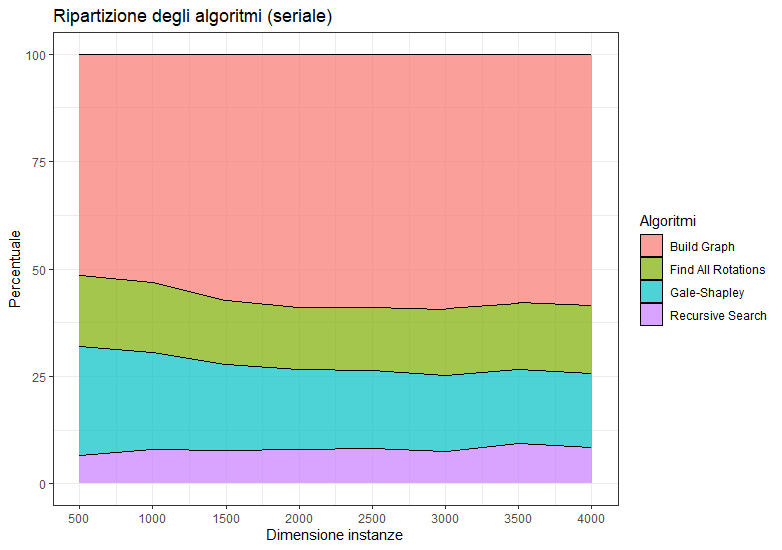
\includegraphics[scale=0.7]{algs_contributes.png}
            \caption{Contributo in percentuale dei vari sotto-algoritmi seriali al tempo totale.}
            \label{fig:contributi}
        \end{figure}
        \FloatBarrier
        
        Si è quindi deciso di implementare una soluzione parallela per velocizzare la parte di programma più costosa in termini di tempo, cioè la costruzione del grafo. Per le altri parti del programma, verranno mantenute le versioni seriali dei vari sotto-algoritmi.

    \subsection{Descrizione generale}
    L'algoritmo parallelo è molto simile a quello seriale, con alcune importanti differenze. In questo paragrafo, ci concentreremo soprattutto su ciò in cui la versione seriale e quella parallela differiscono.
    
    La prima questione da affrontare è stata trovare delle strutture dati appropriate per la versione parallela. Le strutture dati utilizzate all'interno del kernel sono o uguali o molto simili a quelle della controparte seriale, essendo tutte sostanzialmente matrici. Le differenze si trovano soprattutto nelle strutture dati usate nell'input e nell'output. In particolare, sono due i problemi più importanti che abbiamo affrontato nello scegliere queste strutture dati:
    \begin{itemize}
        \item la soluzione seriale fa un grosso uso di puntatori all'interno delle strutture dati, specialmente per quanto riguarda le rotazioni. La versione parallela dovrebbe o utilizzare strutture dati equivalenti che non fanno uso di puntatori, oppure ricostruire da zero tutte le strutture dati all'interno della memoria del device; è evidente che, nella maggior parte dei casi, la prima soluzione è preferibile alla seconda.
        \item ridurre il consumo della memoria del device: la memoria disponibile all'interno del device è molto inferiore a quella che l'host può utilizzare. Questo è un problema importante in quanto la nostra soluzione, e questo problema in generale, richiedono l'uso di molta memoria.
    \end{itemize}
    Abbiamo quindi deciso di sostituire le strutture dati presenti nella versione seriale con altre equivalenti che non fanno uso di puntatori, eliminando inoltre tutte le informazioni non strettamente necessarie a questo passo della computazione e in generale riducendo al minimo la memoria occupata. Dunque, il kernel riceve come input un vettore contiguo contenente tutte le coppie presenti nelle rotazioni e un secondo vettore per permettere di distinguere dove finiscono le coppie di una rotazione e dove iniziano quelle di un'altra. L'output del kernel è invece una semplice matrice triangolare, contenuta in un vettore, che rappresenta le relazioni di dipendenza tra le diverse rotazioni. Queste strutture dati sono spiegate in più dettaglio nel paragrafo \ref{StruttureDatiParallele}. Si noti che, grazie all'utilizzo di questa matrice triangolare, il grafo definito da questa procedura non presenta archi ridondanti, a differenza di quello che viene trovato dalla sua controparte seriale. Va anche sottolineato però che questa differenza non è significativa in quanto, come specificato nel paragrafo \ref{DescrizioneGeneraleSeriale}, con una piccola modifica è possibile rimuovere questa ridondanza anche dalla versione seriale.

    Per supportare l'uso di queste nuove strutture dati, è stato necessario aggiungere al codice host del codice che gestisca l'inizializzazione degli input e l'applicazione dell'output alla struttura dati che rappresenta il grafo nei successivi passi seriali dell'algoritmo. La complessità asintotica di queste operazioni è $O(n^2)$.

    Si è deciso che tutti i thread sarebbero stati eseguiti in \textbf{un unico blocco}. La ragione è che, durante la creazione delle etichette, gli accessi alle caselle della matrice delle etichette avvengono in modo non ordinato, ma secondo le coppie presenti nelle rotazioni: non è quindi possibile suddividere il problema della costruzione del grafo in diversi problemi uguali ma più piccoli e indipendenti fra loro. Se ciò è possibile per la fase di calcolo delle dipendenze fra le rotazioni e può essere ottenuto in qualche modo nella fase di inizializzazione, non è però possibile suddividere l'insieme delle rotazioni in modo che ogni sottoinsieme coinvolga esclusivamente una sezione contigua della matrice delle etichette (lo stesso vale anche per \texttt{label\_second\_condition}).

    Vengono lanciati tanti thread quanto il massimo tra $n$ e il numero di rotazioni, senza comunque superare il limite di 1024 thread che possono essere lanciati nello stesso blocco. La ragione di questi numeri sarà chiara tra poco.

    Il codice del kernel può essere diviso in tre parti: l'inizializzazione delle varie strutture dati ad esso interne, il calcolo della tabelle delle etichette (e di \texttt{label\_second\_condition}) e il calcolo delle dipendenze tra le rotazioni. Dei comandi \texttt{\_\_syncthreads()} dividono le varie sezioni, in quanto ognuna è dipendente dal completamento di tutta la sezione precedente.

    All'inizio dell'esecuzione, tutti i thread aspettano che il thread 0 allochi lo spazio per le strutture dati interne. Seguono quindi diverse fasi di inizializzazione, in cui ad ogni thread sono assegnati degli uomini/donne o delle rotazioni, a seconda della fase, rispetto ai quali inizializzare le strutture dati. Gli uomini/donne e le rotazioni sono suddivisi in modo uguale tra i diversi thread, in modo che, se il loro numero fosse maggiore di 1024, ogni thread cicli su un piccolo sottoinsieme di essi. I thread a cui non è assegnato nulla rimangono in attesa che gli altri finiscano. Vedremo che questo modo di operare sarà utilizzato anche nelle sezioni successive. Tra le varie fasi sono presenti dei comandi \texttt{\_\_syncwarp()} per migliorare la sincronizzazione e quindi l'efficienza dell'esecuzione e da un comando \texttt{\_\_syncthreads()} dove la mancanza di sincronizzazione potrebbe introdurre errori.

    Nella seconda parte del codice del kernel, vengono riempite la matrice contenente le etichette e \texttt{label\_second\_condition}. Il codice è molto simile a quello seriale, riadattato in modo da funzionare con le nuove strutture dati. Ad ogni thread è assegnata una o più rotazioni, a seconda del numero di rotazioni. Il ciclo \texttt{for} principale, ovvero quello che cicla fra tutte le rotazioni assegnate al thread, contiene al suo interno dei comandi \texttt{\_\_syncwarp()}, così assicurare la sincronizzazione tra i thread e migliorare le prestazioni. Per rendere questo possibile, anche i thread a cui in quel particolare ciclo non è assegnata alcuna rotazione entrano all'interno del ciclo \texttt{for}: grazie a degli \texttt{if} questi thread non eseguono alcuna parte della logica interna al ciclo, ma riescono ugualmente a raggiungere i comandi di sincronizzazione, evitando così \textit{deadlock}. Per ottenere ciò, viene calcolato a priori il numero di iterazioni necessarie al ciclo. Si noti che le stesse strategie per la sincronizzazione non sono state impiegate per i cicli interni, in quanto richiederebbero una grande complicazione del codice che difficilmente porterebbe a dei miglioramenti delle prestazioni. Una importante differenza con la versione seriale riguarda il modo in cui viene riempita la matrice delle etichette. L'algoritmo seriale richiede che le rotazioni vengano scansionate in ordine, in modo che nessuna rotazione venga esaminata prima di uno dei suoi predecessori. Inoltre, nell'algoritmo seriale i vettori \texttt{last\_labelled\_man\_index} e \texttt{last\_labelled\_woman\_index} permettono di aggiungere la nuova etichetta partendo dall'ultima donna etichettata per quell'uomo da una delle rotazioni precedenti; questo non è possibile nella nostra soluzione parallela, perché solo un'esecuzione seriale può assicurare che tutte le etichette definite dalle rotazione precedenti siano già state calcolate. La soluzione parallela affronta questo problema scandendo la matrice delle etichette partendo sempre dalla donna associata all'uomo in questione nel top matching. La nuova etichetta viene scritta nella matrice solo se non era presente alcuna etichetta per quella coppia, o se l'etichetta associata a quella coppia identificava una rotazione successiva a quella attuale. Per evitare che accessi concorrenti introducano errori, viene usata l'operazione atomica \texttt{atomicMin()}. Date le grosse dimensioni della matrice delle etichette, è poco probabile che due thread cerchino di eseguire contemporaneamente una operazione atomica sulla stessa cella della matrice. Si noti che in questo modo vengono scansionate (e potenzialmente scritte) molte più etichette che nella versione seriale, in cui invece ogni coppia viene scansionata in questa fase al più una sola volta; la \textbf{complessità} di questa parte dell'algoritmo e, di conseguenza, di tutto l'algoritmo di creazione del grafo, diventa $O(n^3)$ invece che $O(n^2)$.\footnote{La complessità asintotica è calcolata come il numero di passi che vengono eseguiti complessivamente da tutti i thread.}

    Nell'ultima fase del calcolo delle dipendenze, ad ogni thread è assegnato uno o più uomini, usando le stesse strategie di sincronizzazione usate nella fase precedente. Questa sezione dell'algoritmo è probabilmente la più simile alla versione parallela. Le differenze principali sono gli adattamenti necessari per usare le nuove strutture dati e l'utilizzo di una matrice invece di un vettore per memorizzare le rotazioni già applicate rispetto ad un singolo uomo. La seconda modifica è dovuta al fatto che, a causa alla scansione concorrente delle liste di più uomini, non è più possibile usare un singolo vettore che viene resettato al termine della scansione della lista di ogni uomo.

    Una volta che tutti i thread hanno completato anche l'ultima fase, il thread 0 libera la memoria allocata per le strutture dati interne.
    
    \subsection{Le strutture dati}
    \label{StruttureDatiParallele}
    In questo paragrafo sono presentate le strutture dati utilizzate nel codice parallelo. 
    \begin{itemize}
        \item \textbf{triangular\_matrix:} non potendo utilizzare strutture dati dinamiche nella costruzione del grafo, si è dovuto trovare una struttura dati alternativa per rappresentare le dipendenze tra le rotazioni. La rappresentazione scelta è una matrice triangolare inferiore con dimensione pari al numero di rotazioni meno 1. La matrice contiene valori booleani; il booleano nella posizione $(x,y)$ della matrice contiene la risposta alla domanda: \quotes{la rotazione $y+1$ dipende dalla rotazione $x$?}. Si noti che, grazie a questa definizione, ogni casella della matrice identifica una relazione di dipendenza effettivamente possibile. La matrice è memorizzata sotto forma di un unico vettore contiguo, che viene indicizzato secondo la formula $(y-1)*y/2 + x$.\footnote{Si noti che la prima rotazione ha indice $0$.}
        
        Ad esempio, la matrice triangolare per un totale di 5 rotazioni avrebbe la seguente struttura, con $B$ che rappresenta un valore booleano: 

        \begin{center}
            \begin{math}
                \begin{matrix}
                    B & \cdot & \cdot & \cdot \\
                    B & B & \cdot & \cdot \\
                    B & B & B & \cdot \\
                    B & B & B & B \\
                \end{matrix}
            \end{math}
        \end{center}
        
        \item \textbf{rotations\_vector} contiene tutte le coppie di tutte le rotazioni, ordinate secondo l'indice delle rotazioni. Per evitare accessi disallineati alla memoria, la prima metà del vettore contiene solo gli uomini delle coppie delle rotazioni, mentre la seconda metà contiene le donne.
        \item \textbf{end\_displacement\_vector} contiene, per ogni rotazione, l'indice del suo ultimo uomo in \texttt{rotations\_vector}. Per ottenere l'offset delle donne nel vettore, è sufficiente sommare all'indice dell'uomo in numero totale di coppie in tutte le rotazioni.
        \item \textbf{rotation\_vector} contiene nella posizione \texttt{i} il puntatore al \texttt{RotationNode} della \texttt{i}-esima rotazione. È utilizzato per velocizzare l'applicazione dei risultati contenuti nella matrice triangolare ai \texttt{RotationNode} che rappresentano il grafo.
    \end{itemize}

    \subsection{La memoria}
    Come introdotto nei paragrafi precedenti, questo algoritmo ha bisogno di molta memoria. Nelle nostre prove, al crescere di $n$ la memoria disponibile nel dispositivo diventa insufficiente ben prima che i tempi di esecuzione diventino proibitivi. Con l'hardware a nostra disposizione, ossia una Nvidia Rtx 2080 e una Nvidia Rtx 3060, la memoria del dispositivo è sufficiente per eseguire le istanze fino a $n=5049$: per $n>5049$, l'allocazione delle strutture interne fallisce per mancanza di spazio e il programma termina con un errore. Per questo motivo, i confronti con la versione parallela verranno fatti solo per istanze inferiori a questo numero. Inoltre, quando verranno paragonati i tempi necessari per le due soluzioni, va sempre tenuto in mente che la dimensione della memoria della scheda video limita la dimensione massima delle istanze che possono essere eseguite con questo algoritmo. Una scheda video con una maggiore capacità di memoria sarebbe in grado di eseguire su istanze di dimensioni maggiori.

    A causa di questo grande consumo di memoria, non sono state possibili grandi ottimizzazioni riguardo gli accessi alla memoria. Infatti, le strutture dati utilizzate sono di dimensioni tali da dover stare obbligatoriamente in memoria globale. Solo i puntatori alle strutture dati possono stare in una memoria diversa, oltre ovviamente alle variabili intere locali ai singoli thread. I puntatori sono stati dunque messi in memoria shared, per velocizzarne l'accesso. Un altro problema che ha impedito di effettuare grandi miglioramenti è stato il tipo di accesso ai dati effettuato dall'algoritmo: la maggior parte delle locazioni di memoria viene letto al più un paio di volte, solitamente in zone del codice lontane tra loro. Per questo motivo e per la dimensione dei dati, non è stato possibile ottimizzare l'uso della cache. Le inizializzazioni delle strutture dati sono state pensate in modo da allineare gli accessi in scrittura da memoria. Inoltre, come spiegato nel paragrafo \ref{StruttureDatiParallele}, il vettore \texttt{rotation\_vector} è stato strutturato in modo da allineare gli accessi alla memoria.
    
    \subsection{L'algoritmo parallelo}
    In questa sezione, l'algoritmo parallelo viene descritto ad alto livello. Per il codice CUDA effettivo, si rimanda ai file del progetto. Lo pseudocodice lato host contiene solo le parti modificate per le esigenze del codice device; il resto è da intendersi uguale alla versione seriale.

    
    \begin{algorithm}[H]
        \scriptsize
        \DontPrintSemicolon
        \caption{ALL\_STABLE\_MATCHINGS\_CUDA (lato host)}\label{alg:AllStableMatchingsCUDA}
        \KwData{n, men\_preferences, women\_preferences}
        \;
        [...]\;
        \;
        scorre la lista delle rotazioni e la lista delle coppie di ogni rotazione per calcolare il numero totale di rotazioni (\texttt{number\_of\_rotations}) e il numero totale di coppie nelle rotazioni (\texttt{total\_number\_of\_pairs})\;
        \;
        alloca con memoria mapped uno spazio di \texttt{total\_number\_of\_pairs} * 2 interi per \texttt{rotations\_vector}, uno spazio di \texttt{number\_of\_rotations} interi per \texttt{end\_displacement\_vector} e ((\texttt{number\_of\_rotations}-1)*\texttt{number\_of\_rotations})/2 interi per \texttt{triangular\_matrix}\;
        \;
        alloca nella memoria dell'host \texttt{number\_of\_rotations} puntatori a nodi delle rotazioni per \texttt{rotation\_vector}\;
        \;
        scorre nuovamente tutta la lista delle rotazioni e la lista delle coppie di ogni rotazione, così da riempire \texttt{rotations\_vector}, \texttt{end\_displacement\_vector} e \texttt{rotation\_vector}\;
        \;
        mette nella memoria del device il top matching e le preferenze degli uomini e delle donne\;
        \;
        \texttt{//lancio del kernel}\;
        NumThPerBlock = min(max(number\_of\_rotations, n), 1024)\;
        BUILD\_GRAPH\_CUDA$<<<$1, NumThPerBlock$>>>$(n, number\_of\_rotations, total\_number\_of\_pairs, rotations\_vector, end\_displacement\_vector, top\_matching, women\_preferences, dev\_men\_preferences, triangular\_matrix)\;
        \;
        \For{ogni rotazione nella lista delle rotazioni}{
        \For{ogni elemento nella riga di \texttt{triangular\_matrix} relativa alla rotazione}{
        \If{c'è una dipendenza}{
            incrementa di 1 \texttt{missing\_predecessors} della rotazione corrente\;
            aggiungi la rotazione corrente alla lista dei successori della rotazione da cui dipende, che viene reperita indicizzando \texttt{rotation\_vector}\;
        }
        }
        }\;
        libera la memoria\;
        \;
        [...]\;
        \;
    \end{algorithm}

    \begin{algorithm}[H]
        \scriptsize
        \DontPrintSemicolon
        \caption{BUILD\_GRAPH\_CUDA (lato device)}\label{alg:BuildaGraphCUDA}
        \KwData{n, number\_of\_rotations, total\_number\_of\_pairs, rotations\_vector, end\_displacement\_vector, top\_matching, women\_preferences, men\_preferences, triangular\_matrix}
        \;
        //Allocazione della memoria\;
        \If{threadIdx.x == 0}{
            alloca $n^2$ interi per \texttt{label\_matrix}\;
            alloca $n^2$ char per \texttt{is\_stable\_matrix}\;
            alloca $n^2$ char per \texttt{label\_second\_condition}\;
            alloca $number\_of\_rotations * n$ interi per \texttt{applied\_rotations}\;
            alloca $n$ interi per \texttt{first\_men\_preferences\_index}\;
            alloca $n$ interi per \texttt{first\_women\_preferences\_index}\;
        }
        \_\_syncthreads()\;
        \;
        //Inizializzazione delle strutture dati interne\;
        \For{i=threadIdx.x; i$<$n; i+=blockDim.x}{
            inizializza tutti i valori della \texttt{j}-esima riga di \texttt{label\_matrix} a \texttt{number\_of\_rotations} (indica l'assenza di etichette)\;
            inizializza tutti i valori della \texttt{j}-esima riga di \texttt{is\_stable\_matrix} a $False$\;
            inizializza tutti i valori della \texttt{j}-esima riga di \texttt{label\_second\_condition} a $False$\;
        }
        \_\_syncthreads()\;
        \;
        \For{i=threadIdx.x; i$<$n; i+=blockDim.x}{
            is\_stable\_matrix[top\_matching[i]][i]=$True$\;
            \For{j=0; j$<$n; j++}{
                \If{top\_matching[j] == men\_preferences[j][i]}{
                    first\_men\_preferences\_index[j] = i\;
                }
                \If{j == women\_preferences[top\_matching[j]][i]}{
                    first\_women\_preferences\_index[top\_matching[j]] = i\;
                }
            }
        }
        \_\_syncwarp()\;
        \;
        \For{i=threadIdx.x; i$<$number\_of\_rotations; i+=blockDim.x}{
            inizializza tutti i valori della \texttt{j}-esima riga di \texttt{applied\_rotations} a $False$\;
        }
        \_\_syncwarp()\;
        \;
        \For{i = threadIdx.x; i $<$ ((number\_of\_rotations-1)*number\_of\_rotations)/2; i+=blockDim.x}{
            triangular\_matrix[i] = $False$;
        }
        \_\_syncthreads()\;
        \;
        \textit{continua...}
    \end{algorithm}

    \begin{algorithm}[H]
        \scriptsize
        \DontPrintSemicolon
        \texttt{//Calcolo delle etichette}\;
        iterations = ceiling(number\_of\_rotations/blockDim.x)\;
        \For{i=threadIdx.x; i$<$iterations*blockDim.x; i+=blockDim.x}{
            \If{i $<$ number\_of\_rotations}{
                usando \texttt{end\_displacement\_vector}, calcola la posizione del primo uomo della rotazione \texttt{i}-esima in \texttt{rotations\_vector} e assegnalo a \texttt{j}\;
            }
            \_\_syncwarp()\;
            \If{i $<$ number\_of\_rotations}{
                \texttt{first\_woman} è la donna che appare nella prima coppia della \texttt{i}-esima rotazione\;
                \For{j$\le$end\_displacement\_vector[i]; j++}{
                    man = rotations\_vector[j]\;
                    \texttt{next\_woman} = la donna della coppia successiva (\texttt{first\_woman} se è stata raggiunta la fine della rotazione)\;
                    woman = rotations\_vector[total\_number\_of\_pairs+j]\;
                    \;
                    \texttt{//Aggiorna rispetto alle preferenze della donna}\;
                    k = first\_women\_preferences\_index[next\_woman]-1\;
				    \While{women\_preferences[next\_woman][k] $\ne$ man}{
					   atomicMin(label\_matrix[next\_woman][women\_preferences[next\_woman][k]],i)\;
					   k--\;
				    }
                    \texttt{//Aggiorna rispetto alle preferenze dell'uomo}\;
                    k = first\_men\_preferences\_index[man]+1\;
				    \While{men\_preferences[man][k] $\ne$ next\_woman}{
				    	label\_second\_condition[man][men\_preferences[man][k]]=$True$\;
				    	k++\;
				    }
                    \;
                    is\_stable\_matrix[next\_woman][man]=$True$\;
				    atomicMin(label\_matrix[woman][man],i)\;
                }
            }
            \_\_syncwarp()\;
        }
        \_\_syncthreads()\;
        \;
        \texttt{//Calcolo delle dipendenze}\;
        iterations = ceiling(n/blockDim.x)\;
        \For{man = threadIdx.x; man $<$ iterations*blockDim.x; man += blockDim.x}{
            \If{man $<$ n}{
                k = 0\;
                \While{top\_matching[man] $\ne$ men\_preferences[man][k]}{
				    k++\;
                }
            }
            \_\_syncwarp()\;
            \If{man $<$ n}{
                p\_star = -1\;
                \For{j = k; j $<$ n; j++}{
                    woman = men\_preferences[man][j]\;
                    \If{la coppia (\texttt{woman},\texttt{man}) non è etichettata}{
                        continue\;
                    }
                    \texttt{//Etichetta di tipo 1}\;
                    \If{is\_stable\_matrix[woman][man]}{
                        \If{p\_star $\ne$ -1}{
                            triangular\_matrix[(label\_matrix[woman][man]-1)*number\_of\_rotations+p\_star]=$True$\;
                        }
                        p\_star = label\_matrix[woman][man]\;
                        applied\_rotations[man][label\_matrix[woman][man]] = $True$\;
                    }
                    \texttt{//Etichetta di tipo 2}\;
                    \ElseIf{$\neg$applied\_rotations[man][label\_matrix[woman][man]] $\land$ label\_second\_condition[man][woman]}{
                        triangular\_matrix[p\_star-1][label\_matrix[woman][man]] = $True$\;
                        applied\_rotations[man][label\_matrix[woman][man]] = $True$\;
                    }
                }
            }
            \_\_syncwarp()\;
        }
        \_\_syncthreads()\;
        \;
        il thread 0 libera la memoria che aveva allocato\;
    \end{algorithm}

    \subsection{Possibili miglioramenti}
    \label{PossibiliMiglioramenti}
    Sono possibili diversi approcci per provare a migliorare le prestazioni di questo algoritmo parallelo.

    In primo luogo, cambiando la rappresentazione dei dati usati dai sotto-algoritmi seriali, in modo che sia la stessa usata dal sotto-algoritmo parallelo, sarebbe possibile ridurre gli overhead per la conversione dei dati di input e output.

    Per rendere possibile l'utilizzo dell'algoritmo parellelo su istanze più grandi, si potrebbero tentare nuove strategie per ridurre ulteriormente l'uso della memoria sul device. Alcune di queste strategie potrebbero ridurre l'uso della memoria a discapito della semplicità del codice, rendendolo più complesso sia in termini di righe di codice che di numero di operazioni che devono essere eseguite. Si sottolinea, in questo contesto, che CUDA non permette operazioni atomiche su tipi di dati più piccoli di 32 bit, per cui per trasformare \texttt{label\_matrix} in una matrice di \texttt{short} invece che di \texttt{int} sarebbe necessario implementare una alternativa ad \texttt{atomicMin()}. Sono stati fatti dei veloci tentativi di utilizzare, per alcune strutture dati, \texttt{short} invece che \texttt{int}, senza però ottenere miglioramenti riguardo la dimensione dell'istanza più grande che il dispositivo riesce a gestire; ulteriori approfondimenti sarebbero necessari.

    Per quanto sia molto difficile che porti a miglioramenti, data la grossa dimensione delle matrici rispetto a quella piuttosto limitata della cache L2, si potrebbe provare a dare maggiore priorità nella cache alle due matrici delle preferenze, essendo esse lette più frequentemente delle altre strutture dati.

    Se non ci fossero le limitazioni della memoria del device che abbiamo riscontrato, si potrebbe aumentare la parallelizzazione separando la fase di riempimento della matrice delle etichette da quella di calcolo delle dipendenze. In questo modo, eseguendo le due fasi con kernel distinti, sarebbe possibile eseguire i thread in blocchi separati, in quanto non sarebbero più necessarie sincronizzazioni tra i kernel della stessa grid. Potrebbe essere necessario spostare anche la fase di inizializzazione delle strutture dati su un kernel separato. Con le limitazioni riscontrate con i device a nostra disposizione, difficilmente gli overhead potrebbero giustificare un approccio di questo tipo.

    Descriviamo infine un approccio che potrebbe permettere di utilizzare questo algoritmo nonostante i limiti di memoria. Si potrebbero lanciare in successione diverse grid di thread, ad ognuna delle quali viene assegnato un determinato numero di righe adiacenti della matrice delle etichette (e di \texttt{label\_second\_condition}), ovvero una sezione della matrice la cui dimensione non supera lo spazio disponibile nel device. Ogni thread si occuperebbe di scansionare una delle righe assegnate al grid e le matrici triangolari calcolate dalle diverse grid andrebbero unite usando degli \texttt{OR}. Se i thread facessero tutti parte dello stesso blocco, sarebbe possibile far calcolare ad ogni grid la parte di matrice di cui ha bisogno, rieseguendo ogni volta l'algoritmo per calcolare tutta la matrice ma effettuando solo le operazioni di scrittura relative alla zona della matrice pertinente a quella grid; una alternativa, probabilmente migliore, sarebbe calcolare lato host la matrice delle etichette, in modo che ogni grid non debba ricalcolarla, il che renderebbe possibile eseguire i thread anche su blocchi diversi. Va comunque sottolineato che, a causa delle limitazioni della memoria, i miglioramenti ottenibili eseguendo i thread su più blocchi sarebbero ridotti: ad ogni thread, infatti, vengono al momento assegnate al più 5 righe ($5049/1024=4,93$ identifica il limite superiore $5$), il che implica che il miglioramento delle prestazioni ottenuto distribuendo i thread su più blocchi non può essere superiore ad un fattore di 5.
    
    Un ultimo approccio che si può sperimentare è di dividere le coppie delle rotazioni a seconda della zona della matrice delle etichette che influenzano, in modo da poter applicare la prima versione della variazione precedente scansionando esclusivamente gli elementi delle rotazioni che modificano la sezione della matrice delle etichette assegnata al grid.

\pagebreak

\section{Risultati sperimentali e osservazioni}
    In questa sezione analizziamo i risultati sperimentali che abbiamo ottenuto, confrontando la versione seriale con quella parallela, con l'ausilio di grafici esplicativi. Sono stati generati 10 campioni casuali da 50 istanze, per $n$ da $500$ a $5000$ con passi da 500; entrambe le versioni sono state valutate con gli stessi campioni. Prima però occorre descrivere le specifiche del dispositivo sul quale sono stati effettuati i test. I test sono stati eseguiti sul sistema operativo Windows 11, mentre le specifiche hardware sono riassunte in tabella \ref{tabella2}:

    \begin{table}[h]
    \centering
    \begin{tabular}{|l|l|l|}
        \hline
        & \textbf{AMD Ryzen 5700G} & \textbf{nVidia GeForce RTX 3060} \\
        \hline
        \textbf{Cores} & 8 & 3584 CUDA cores \\
        \hline
        \textbf{Clock base/boost} & 3.8GHz/4.6GHz & 1320MHz/1777MHz \\
        \hline
        \textbf{FLOPS} & 460.7GFLOPS & 12.74TFLOPS \\
        \hline
        \textbf{Cache} & 4+16MB (L2+L3) & 3MB (L2) \\
        \hline
        \textbf{Memoria} & 32GB & 12GB \\
        \hline
        \textbf{Tipo memoria} & DDR4 & GDDR6 \\
        \hline
    \end{tabular}
    \caption{Specifiche hardware su cui sono stati effettuati i test.}
    \label{tabella2}
    \end{table}

    \FloatBarrier

    Analizziamo come prima cosa i tempi impiegati dalle versioni. I grafici \ref{fig:tempitotali}, \ref{fig:buildgraph} e la tabella \ref{tabella3} mostrano come ci sia stata una importante diminuzione dei tempi. La versione parallela all'incirca dimezza i tempi totali della versione seriale. Invece \texttt{Build Graph} parallelo, paragonato a quello seriale, mostra per le dimensioni considerate un andamento addirittura lineare invece che quadratico, con un miglioramento di un fattore maggiore di 5 per la dimensione massima considerata.

    \begin{figure}[h]
        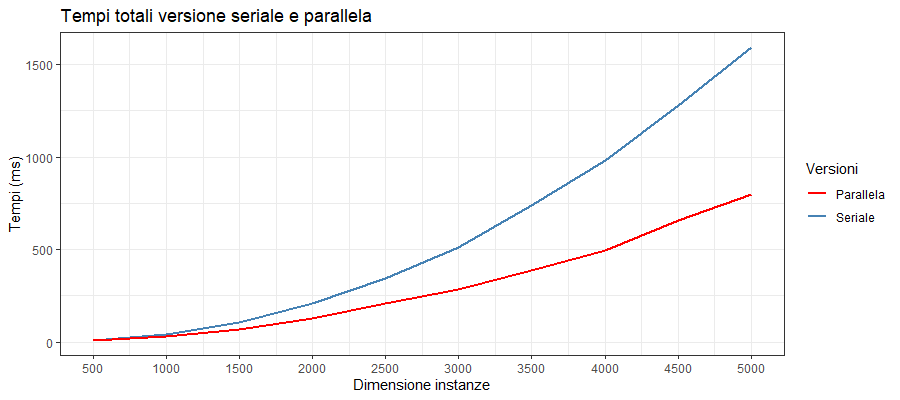
\includegraphics[scale=0.7]{total_times_comparison.png}
        \caption{Comparazione dei tempi totali delle due versioni.}
        \label{fig:tempitotali}
    \end{figure}

    \begin{figure}[h]
        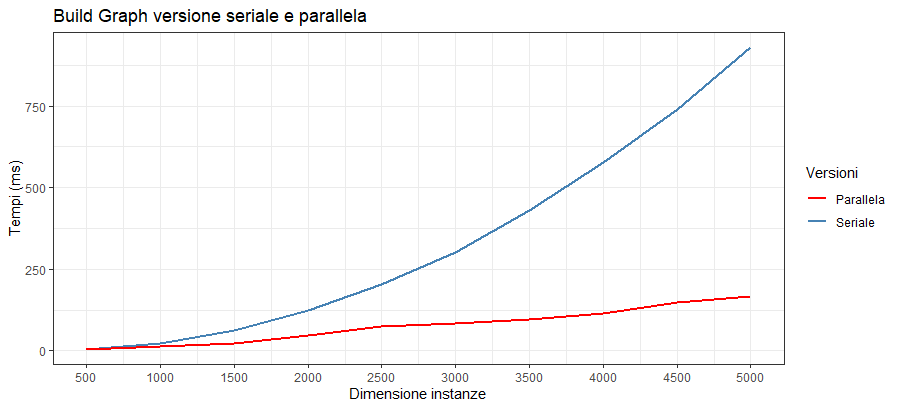
\includegraphics[scale=0.7]{build_graph_comparison.png}
        \caption{Comparazione delle due versioni di Build Graph.}
        \label{fig:buildgraph}
    \end{figure}
    
    \FloatBarrier

    \begin{table}[h]
    \begin{tabular}{|c|c|c|c|c|}
        \hline
        \textbf{n} & \textbf{Tot. seriale} & \textbf{Tot. parallela} & \textbf{Build Graph seriale} & \textbf{Build Graph parallela} \\
        \hline
        500 & 8.86 & 7.38 &  4.46 & 4.36 \\
        \hline
        1000 & 40.90 & 29.08 & 21.72 & 11.68 \\
        \hline
        1500 & 107.42 & 67.24 & 61.68 & 23.78 \\
        \hline
        2000 & 208.48 & 128.36 & 122.78 & 46.04 \\
        \hline
        2500 & 343.74 & 208.28 & 203.76 & 74.24 \\
        \hline
        3000 & 509.52 & 284.24 & 301.92 & 84.62 \\
        \hline
        3500 & 738.70 & 387.96 & 429.28 & 94.48 \\
        \hline
        4000 & 979.86 & 497.60 & 577.22 & 114.32 \\
        \hline
        4500 & 1279.42 & 657.18 & 739.42 & 148.36 \\
        \hline
        5000 & 1593.52 & 799.02 & 928.66 & 165.54 \\
        \hline
        \end{tabular}
    \caption{Dati relativi alle misurazioni effettuate.}
    \label{tabella3}
    \end{table}

    \FloatBarrier

    I prossimi due grafici mostrano il contributo dei diversi sotto-algoritmi nei tempi totali. È chiaro come, nella versione parallela, il tempo impiegato dalla costruzione del grafo sia nettamente diminuito, al punto che ora altri due sotto-algoritmi sono significativamente più lenti. 
        
    \begin{figure}[h]
        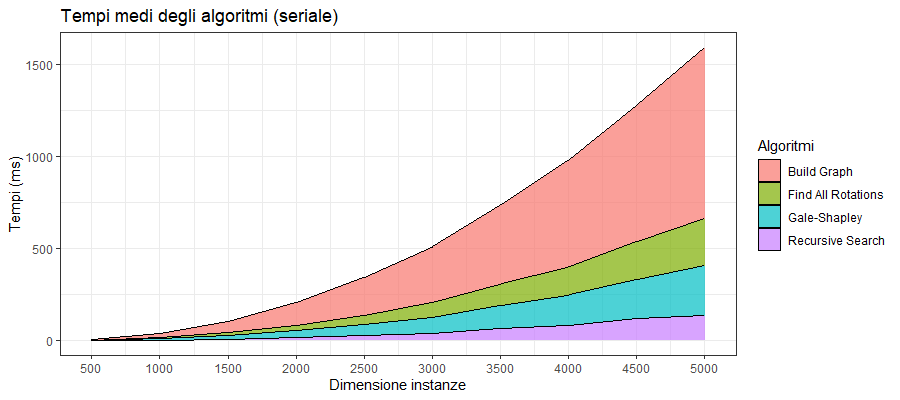
\includegraphics[scale=0.7]{mean_times_serial.png}
        \caption{Tempi medi degli algoritmi della versione seriale.}
        \label{fig:tempimediseriale}
    \end{figure}

    \begin{figure}[h]
        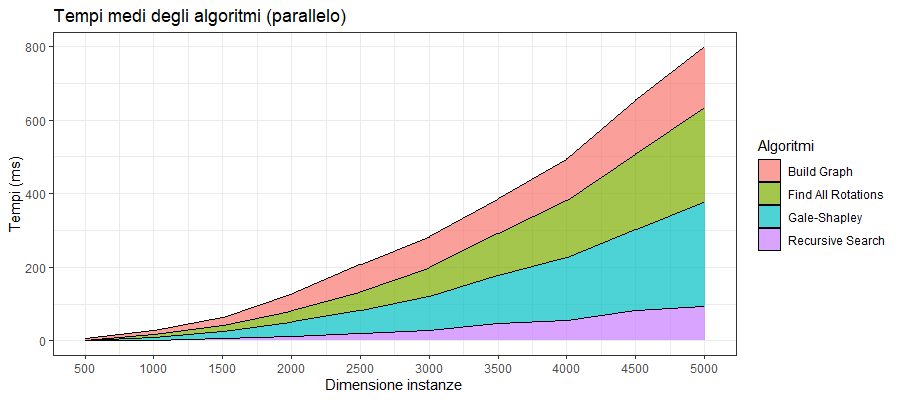
\includegraphics[scale=0.7]{mean_times_parallel.png}
        \caption{Tempi medi degli algoritmi della versione parallela.}
        \label{fig:tempimediparallela}
    \end{figure}

    \FloatBarrier

    Nel paragrafo \ref{PossibiliMiglioramenti} è stato accennato che l'algoritmo potrebbe essere ulteriormente velocizzato modificando i sotto-algoritmi seriali in modo che usino le stesse strutture dati dell'algoritmo parallelo. Il seguente grafico mostra come il kernel e l'overhead per la conversione e il trasferimento dei dati contribuiscono ai tempi totali per la costruzione del grafo. È evidente dal grafico che anche annullando completamente i tempi dell'overhead, cosa impossibile, il miglioramento dei tempi totali sarebbe marginale.

    \begin{figure}[h]
        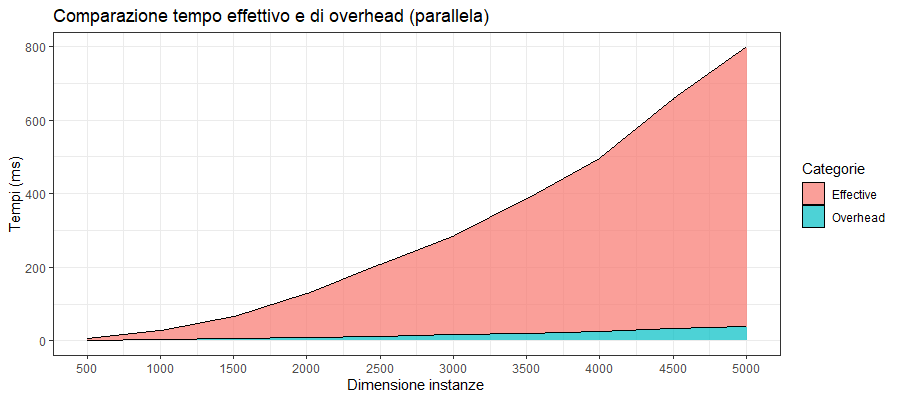
\includegraphics[scale=0.7]{immagini/mean_times_effective_overhead.png}
        \caption{Comparazione tra tempi medi di esecuzione effettiva del kernel e di overhead.}
        \label{fig:tempikerneleffetticooverhead}
    \end{figure}

    \FloatBarrier

    Concludiamo questa sezione con una osservazione. Da tutti i campioni è stata tolta la prima misurazione dei tempi, in quanto includeva un tempo di \quotes{warm up} di \textbf{circa 2 secondi}. Il tempo di esecuzione di una singola istanza della versione parallela è dunque di circa 2 secondi superiore a quello appena mostrato. È possibile però migliorare le prestazioni lanciando in modo asincrono un kernel di \quotes{warm up}, che renda la GPU immediatamente disponibile al kernel successivo.
    
\pagebreak

\section{Istruzioni di compilazione}
    Di seguito si illustrano le istruzioni per la compilazione del progetto. Vista la complessità del problema, si è reso necessario l'utilizzo di un \texttt{Makefile} per aiutare l'utente nella compilazione ed esecuzione. Inoltre, si vuole evidenziare che è stato necessario testare il progetto sotto diversi \virg{punti di vista}, per avere una misura quantomeno accettabile della correttezza. Prima di proseguire con la spiegazione dei comandi presenti nel Makefile, è doveroso fare alcune premesse:

    \begin{itemize}
        \item Il Makefile si trova all'interno della directory \texttt{$\backslash$src}, pertanto è necessario posizionarsi all'interno di quella directory prima di lanciare i comandi che si illustreranno a breve. 
        \item Il Makefile è stato scritto con sintassi per Windows; ciò significa che i comandi genereranno errori se eseguiti all'interno di ambienti diversi, come per esempio UNIX.
        \item Sono stati utilizzati i compilatori \textbf{gcc} per la parte seriale e \textbf{nvcc} per la parte parallela. Ogni comando del Makefile si occupa di compilare e richiamare il relativo eseguibile automaticamente.
    \end{itemize}

    Fatte le dovute precisazioni si può passare a descrivere ciascun comando presente all'interno del Makefile. Si noti che per questioni di spazio, gli argomenti di ogni comando verranno scritti su righe diverse, ovviamente a terminale vanno scritti di seguito separati da spazio.\\

    \textbf{Test su istanze singole}: il primo passo per poter verificare la correttezza del programma è quello di testare singole specifiche istanze. Esempi di istanze di questo tipo si trovano nella directory \texttt{$\backslash$tests}. All'interno si trovano file con estensione .txt contenenti in ordine: dimensione istanza (n), matrice di preferenze degli uomini e matrice di preferenze delle donne. I nomi di alcuni file sono auto-esplicativi ma in linea di massima la directory contiene istanze semplici (1, 2 o 3 soluzioni previste come output) e istanze più complesse, come quelle dei paper scientifici, grazie alle quali si è potuto verificare se i nostri output fossero uguali a quelli presentati nei paper. Nel Makefile sono presenti quindi due comandi \texttt{make} a tal proposito, uno per la parte seriale e l'altro per la parte parallela. In entrambi i casi, è necessario passare il file di input e indicare il file di output dove verranno stampati i risultati (se non presente, verrà creato automaticamente). Esempi di comandi di questo tipo possono essere:

    \begin{table}[h]
    \begin{tabular}{lll}
        \texttt{make} & \texttt{serial} & \texttt{input\_file=..$\backslash$tests$\backslash$1solution.txt} \\ 
        & & \texttt{output\_file=output$\backslash$serial\_tests$\backslash$output.txt} \\
        \end{tabular}
    \end{table}

    \begin{table}[h]
    \begin{tabular}{lll}
        \texttt{make} & \texttt{parallel} & \texttt{input\_file=..$\backslash$tests$\backslash$1solution.txt} \\ 
        & & \texttt{output\_file=output$\backslash$parallel\_tests$\backslash$output.txt} \\
        \end{tabular}
    \end{table}

    \textbf{Test su istanze multiple generate casualmente}: il passo successivo è generalizzare il test su istanze singole a istanze multiple casuali. \'E necessario quindi specificare la dimensione di ciascuna istanza da generare, il numero di iterazioni o test da effettuare e il file di output dove verranno stampati i risultati. Inoltre, bisogna specificare una modalità di output che può essere di due tipi: 
    
    \begin{itemize}
        \item \textbf{classic} il file .txt di output conterrà nella prima colonna il tempo necessario a calcolare le soluzioni, nella seconda colonna il numero di soluzioni trovate e nella terza la dimensione delle istanze.
        \item \textbf{times} Nella versione seriale il file .txt di output conterrà nelle prime 4 colonne i tempi di ogni sotto-algoritmo e nell'ultima il tempo totale per calcolare le soluzioni. Nella versione parallela, la colonna relativa ai tempi di Build Graph è sostituita dalle colonne relative ai tempi di esecuzione del kernel, di overhead e della somma dei due.
    \end{itemize}
    
    Vi è un ultimo argomento opzionale che si può passare ed è il seme dal quale verranno generate le istanze casuali. Se non viene specificato, viene utilizzato un seme di default. Anche in questo caso, vi è un comando per la versione seriale e uno per la versione parallela. Esempi di comandi di questo tipo possono essere:

    \begin{table}[h]
    \begin{tabular}{lll}
        \texttt{make} & \texttt{tester} & \texttt{instance=100} \\ 
        & & \texttt{iterations=100} \\
        & & \texttt{mode=classic} \\
        & & \texttt{output\_file=output$\backslash$output.txt} \\
        & & \texttt{seed=9}
        \end{tabular}
    \end{table}

    \begin{table}[h]
    \begin{tabular}{lll}
        \texttt{make} & \texttt{cuda\_tester} & \texttt{instance=100} \\ 
        & & \texttt{iterations=100} \\
        & & \texttt{mode=times} \\
        & & \texttt{output\_file=output$\backslash$output.txt} \\
        \end{tabular}
    \end{table}

    \textbf{Analisi dei tempi}: Per effettuare le stesse misurazioni illustrate nelle sezioni precedenti, sono previsti i comandi \texttt{make serial\_analysis} e \texttt{make parallel\_analysis}. Come si può intuire, entrambi i comandi richiamano le rispettive versioni del tester, con argomenti impostati da noi. In particolare, le dimensioni delle istanze vanno da 500 a 5000, con step di 500. Le iterazioni sono 51, la modalità è \texttt{times} e i file di output vengono scritti rispettivamente in \texttt{$\backslash$output$\backslash$serial\_tests$\backslash$} e \texttt{$\backslash$output$\backslash$parallel\_tests$\backslash$}. \\

    \textbf{Comparazione degli output delle due versioni}: come ulteriore prova di correttezza, è previsto anche un comando che si occupa di controllare che i risultati provenienti dalle due versioni siano esattamente gli stessi, sia in termini di numeri, che in termini di composizione dei singoli matching stabili. Se viene trovato un errore durante il controllo, vengono riportate su console le informazioni principali (matrici di preferenze, output seriale e parallelo) e l'esecuzione termina immediatamente. Bisogna passare la dimensione delle istanze da generare, le iterazioni ed eventualmente il seed. Il comando è 

    \begin{table}[h]
    \begin{tabular}{lll}
        \texttt{make} & \texttt{comparator} & \texttt{instance=100} \\ 
        & & \texttt{iterations=50} \\
        \end{tabular}
    \end{table}
    
    \textbf{demo}: è stata predisposta una demo (\texttt{make demo}) funzionante del programma con parametri fissati che si occupa di effettuare chiamate multiple a solutions\_comparator. In particolare, la dimensione delle istanze vanno da 500 a 4000 con step di 500, le iterazioni sono 50 e il seed è quello di default. \\

    \textbf{Pulizia di file inutili}: è previsto un ultimo comando \texttt{make clean} per la pulizia di file oggetto, eseguibili, ecc. \\

    Si noti infine che tra i sorgenti vi è il file \texttt{$\backslash$correctness\_tester.c} per il quale non è stato previsto un comando nel makefile. Il motivo è che tale file è stato impiegato solamente a scopo di debug una volta terminata l'implementazione seriale. In particolare si effettua un controllo sui risultati ottenuti dall'esecuzione seriale del nostro programma con i risultati dell'implementazione na\"ive, la quale consiste nell'enumerazione di tutti i matching possibili (stabili e non) e per ognuno, si controlla la condizione di stabilità. Si può facilmente intuire che per motivi di tempistiche dovute alla complessità, la dimensione delle istanze testabili difficilmente supera n=12. Per compilare ed eseguire bisogna digitare i comandi \\

    \texttt{gcc correctness\_tester.c -o correctness}\\

    \texttt{.$\backslash$correctness 3 5}
\pagebreak

\printbibliography

\end{document}